\documentclass{article}

% Language setting
% Replace `english' with e.g. `spanish' to change the document language
\usepackage[english]{babel}

% Set page size and margins
% Replace `letterpaper' with `a4paper' for UK/EU standard size
\usepackage[letterpaper,top=2cm,bottom=2cm,left=3cm,right=3cm,marginparwidth=1.75cm]{geometry}

% Useful packages
\usepackage{amsmath}
\usepackage{graphicx}
\usepackage[colorlinks=true, allcolors=blue]{hyperref}

\title{INFO1111: Computing 1A Professionalism

2023 Semester 1 Self-Learning Report and skills
Level A,B,C
}
\author{ID:  500318346}

\begin{document}
\maketitle

\begin{abstract}
https://github.com/Blackhistoryw/Info1111-
\end{abstract}

\section{Topic: JavaScript}

Topic Overview:

JavaScript is a programming language predominantly used in implementing behavior in webpages and websites. It is used in conjunction with HTML and CSS in which these three tools are used in almost every website or webpage. Web page behavior can include features such as display user-specific information, animate three-dimensional graphics or receiving various types of input from the user. JavaScript is a high-level programming language that is primarily used for creating interactive and dynamic web pages. It is one of the core technologies of the World Wide Web and is supported by all modern web browsers. JavaScript allows developers to add functionality to websites by enabling them to manipulate web page elements, handle events, interact with users, and modify the content of web pages in real-time. JavaScript is characterized by its dynamic typing, which means variables can hold values of any type, and its prototype-based object-oriented programming model. It supports a wide range of programming paradigms, including imperative, functional, and event-driven programming. With JavaScript, I can perform various tasks such as form validation, creating interactive maps, implementing animations and transitions, fetching data from servers asynchronously (Ajax), and building web applications and games. It has a rich ecosystem of libraries, frameworks, and tools, such as React, Angular, Vue.js, and Express.js, which extend its capabilities and make development more efficient.


\section{Application to be developed}

I will develop a webpage with HTML, CSS and JavaScript for create a TV show website using JavaScript. This program will have different sections to add name of different animation and TV, create pics and videos with information of the title users searched. The user will be able to traverse through different sections of the videos through a navigation bar.


\section{Level A/B/C Submission}

\subsection{Learning Approach}

I first approached learning JavaScript by  starting  the  JavaScript  beginner  track  by Youtube, here I learnt a good foundational understanding of JavaScript and how to start programming in it. After watching a part of the online video, I would pause and write my understanding of the  point  explained.  Treehouse also had  quizzes  and programming exercises in which I answered multiple choice questions about what I learnt and programmed some simple JavaScript in their online coding environment.

\subsubsection{}section{Start with the Basics:}

The first step to learning JavaScript is understanding the basics of the language.
Resources:
\begin{itemize}
\item	"JavaScript for Cats": An introduction for new programmers.
\item	"Eloquent JavaScript": A book about JavaScript and programming.
Key Topics:
\item	Variables and Data Types.
\item	Operators (Arithmetic, Assignment, Comparison, Logical, Bitwise).
\item	Control Flow (If..Else, Switch, For, While, Do-While).
\item	Functions and Scope.
\item	Arrays and Objects.
\item	Errors and Exception Handling.
\end{itemize}

\subsubsection{Understanding the Document Object Model (DOM)}

The DOM is a programming interface for web documents. It represents the structure of a document and allows a way to manipulate its content and visual presentation.
Resources:
\begin{itemize}
\item	"DOM Enlightenment": Exploring the relationship between JavaScript and the modern HTML DOM.
\item	Mozilla Developer Network (MDN) DOM Documentation: Comprehensive documentation on the DOM.
Key Topics:
\item	Selecting Elements.
\item	Changing Elements.
\item	Adding and Deleting Elements.
\item	Document and Element properties.
\item	Event Handling.
\end{itemize}

\subsubsection{Dive into Advanced Concepts}

After grasping the basics, I try to learn the more complex aspects of JavaScript.
Resources:
\begin{itemize}
\item	"You Don’t Know JS": A book series which dives deep into the core mechanisms of JavaScript.
\item	"JavaScript: The Good Parts": This book covers the better parts of JavaScript.
Key Topics:
\item	Closures.
\item	Prototypes and Inheritance.
\item	Promises and Async/Await.
\item	ES6+ features like Arrow Functions, Template Literals, Destructuring Assignment, etc.
\item	AJAX (Asynchronous JavaScript and XML).
\end{itemize}

\subsubsection{Practice Skills}

Learning programming isn't just about understanding the concepts. I also need to apply what I've learned.
Resources:
\begin{itemize}
\item	Codecademy: Offers interactive coding exercises with instant feedback.
\item	LeetCode: Focus on solving algorithm problems.
\item	FreeCodeCamp: Offers a full curriculum including a JavaScript algorithm scripting section.
\end{itemize}

\subsubsection{Learn a JavaScript Framework}

I explore JavaScript frameworks which make it easier to build complex applications.
Choose between:
\begin{itemize}
\item	React: Maintained by Facebook, used for building user interfaces, especially for single page applications.
\item	Angular: Maintained by Google, a complete framework including a lot of features out of the box.
\item	Vue.js: Easier to grasp for beginners, lightweight, and versatile.
\end{itemize}

\subsubsection{Build Projects}

Building my own projects not only helps solidify my skills, but also gives me something to show to potential employers.
Possible Project Ideas:
\begin{itemize}
\item	A ToDo List Application.
\item	A Simple Calculator.
\item	A Weather Forecast App using an API.
\end{itemize}


\section{Challenges and Difficulties}

Something I found difficult when learning JavaScript was interacting with HTML and CSS elements, it was difficult to find right functions and syntax to do exactly what I wanted. I found that I had to broaden my understanding of HTML and CSS to fully understand	niche	JavaScript	code. Another element of  learning  JavaScript  I  found  difficult  was understanding how memory and data was stored in the program. I needed to have data saved in the program when switching from my one page to my another page. I tried many methods until I came across local storage and had further difficulties trying to understand the difference between local and session storage.

\section{Create an online TV series viewing website}

\subsection{Plan and design the website}

Determine the structure and layout of the website. Decide on the pages I want to include, such as the homepage, episode list, cast and crew information, and individual episode pages. Sketch out the design or create a wireframe to visualize the website's structure.

\subsection{HTML structure}

Create the basic HTML structure of my website. Each page should have its own HTML file. Use HTML tags to define the structure of my content, such as headings, paragraphs, lists, and links. Include CSS stylesheets to control the visual presentation of the website.

\subsection{CSS styling}

Apply CSS styles to make my website visually appealing. Use CSS rules to define fonts, colors, layout, and other visual properties. Consider using CSS frameworks like Bootstrap or Bulma to simplify styling and make my website responsive across different devices.

\subsection{JavaScript interactivity}

Use JavaScript to add interactivity and dynamic functionality to your website. Here are some examples of how JavaScript can enhance a TV show website:
\begin{itemize}
\item 	Navigation: Implement a navigation menu that allows users to move between different pages of your website without page reloads. You can use JavaScript event handlers, such as click or mouseover, to handle user interactions and update the content dynamically.
\item	Search functionality: Create a search feature that enables users to search for specific episodes or information about the TV show. Implement a search input field and use JavaScript to handle the search queries and filter the results.
\item	Episode list: Fetch episode data from a server or store it locally as JSON objects. Use JavaScript to dynamically generate the episode list based on the data. You can create HTML elements programmatically, add event listeners to handle clicks on individual episodes, and update the content dynamically.
\item	Media playback: If you want to include videos or trailers on your website, you can use JavaScript libraries like Plyr or Video.js to embed and control the playback of media files.
\item	Interactive features: Add interactive elements like quizzes, polls, or user reviews using JavaScript. You can use JavaScript to handle user input, validate form data, and display interactive content based on user interactions.
\end{itemize}

\subsection{Backend functionality}

Depending on the requirements of your website, you may need server-side functionality to handle user authentication, database operations, or external API integrations. For this, you can use server-side frameworks like Node.js with Express or any other backend technology of the choice.

\subsection{Testing and optimization}

Test my website across different browsers and devices to ensure it functions properly and looks good. Optimize the performance of my website by minifying CSS and JavaScript files, optimizing images, and following best practices for web development. Building a complete TV show website involves not only JavaScript but also HTML, CSS, and potentially server-side programming. It's also helpful to explore JavaScript libraries and frameworks that can streamline development and provide ready-made components for certain functionalities.

\section{Learning Sources}

W3schools timing events: \url{https://www.w3schools.com/js/js_timing.asp}

Stack Overflow Forums: \url{https://stackoverflow.com/questions/tagged/javascript}

Youtube: \url{https://www.youtube.com/watch?v=PkZNo7MFNFg&ab_channel=freeCodeCamp.org}

MDN web docs: \url{https://developer.mozilla.org/en-US/search?q=JavaScript}

\section{Application artifacts}

I have made a simple web program with multiple pages. In the pages, the program accepts two user inputs and lookups. The program checks if the user input is valid, and if it is, the program will put the video and URL, and juxtapose the descriptions in a list. The most recent record is displayed at the top of the list. Finally, the user can clear the data with a button on the page. My project folder is attached to this submission.

\url{https://github.com/Blackhistoryw/Info1111- }
code in link 

\section{Screenshots}

\begin{figure}
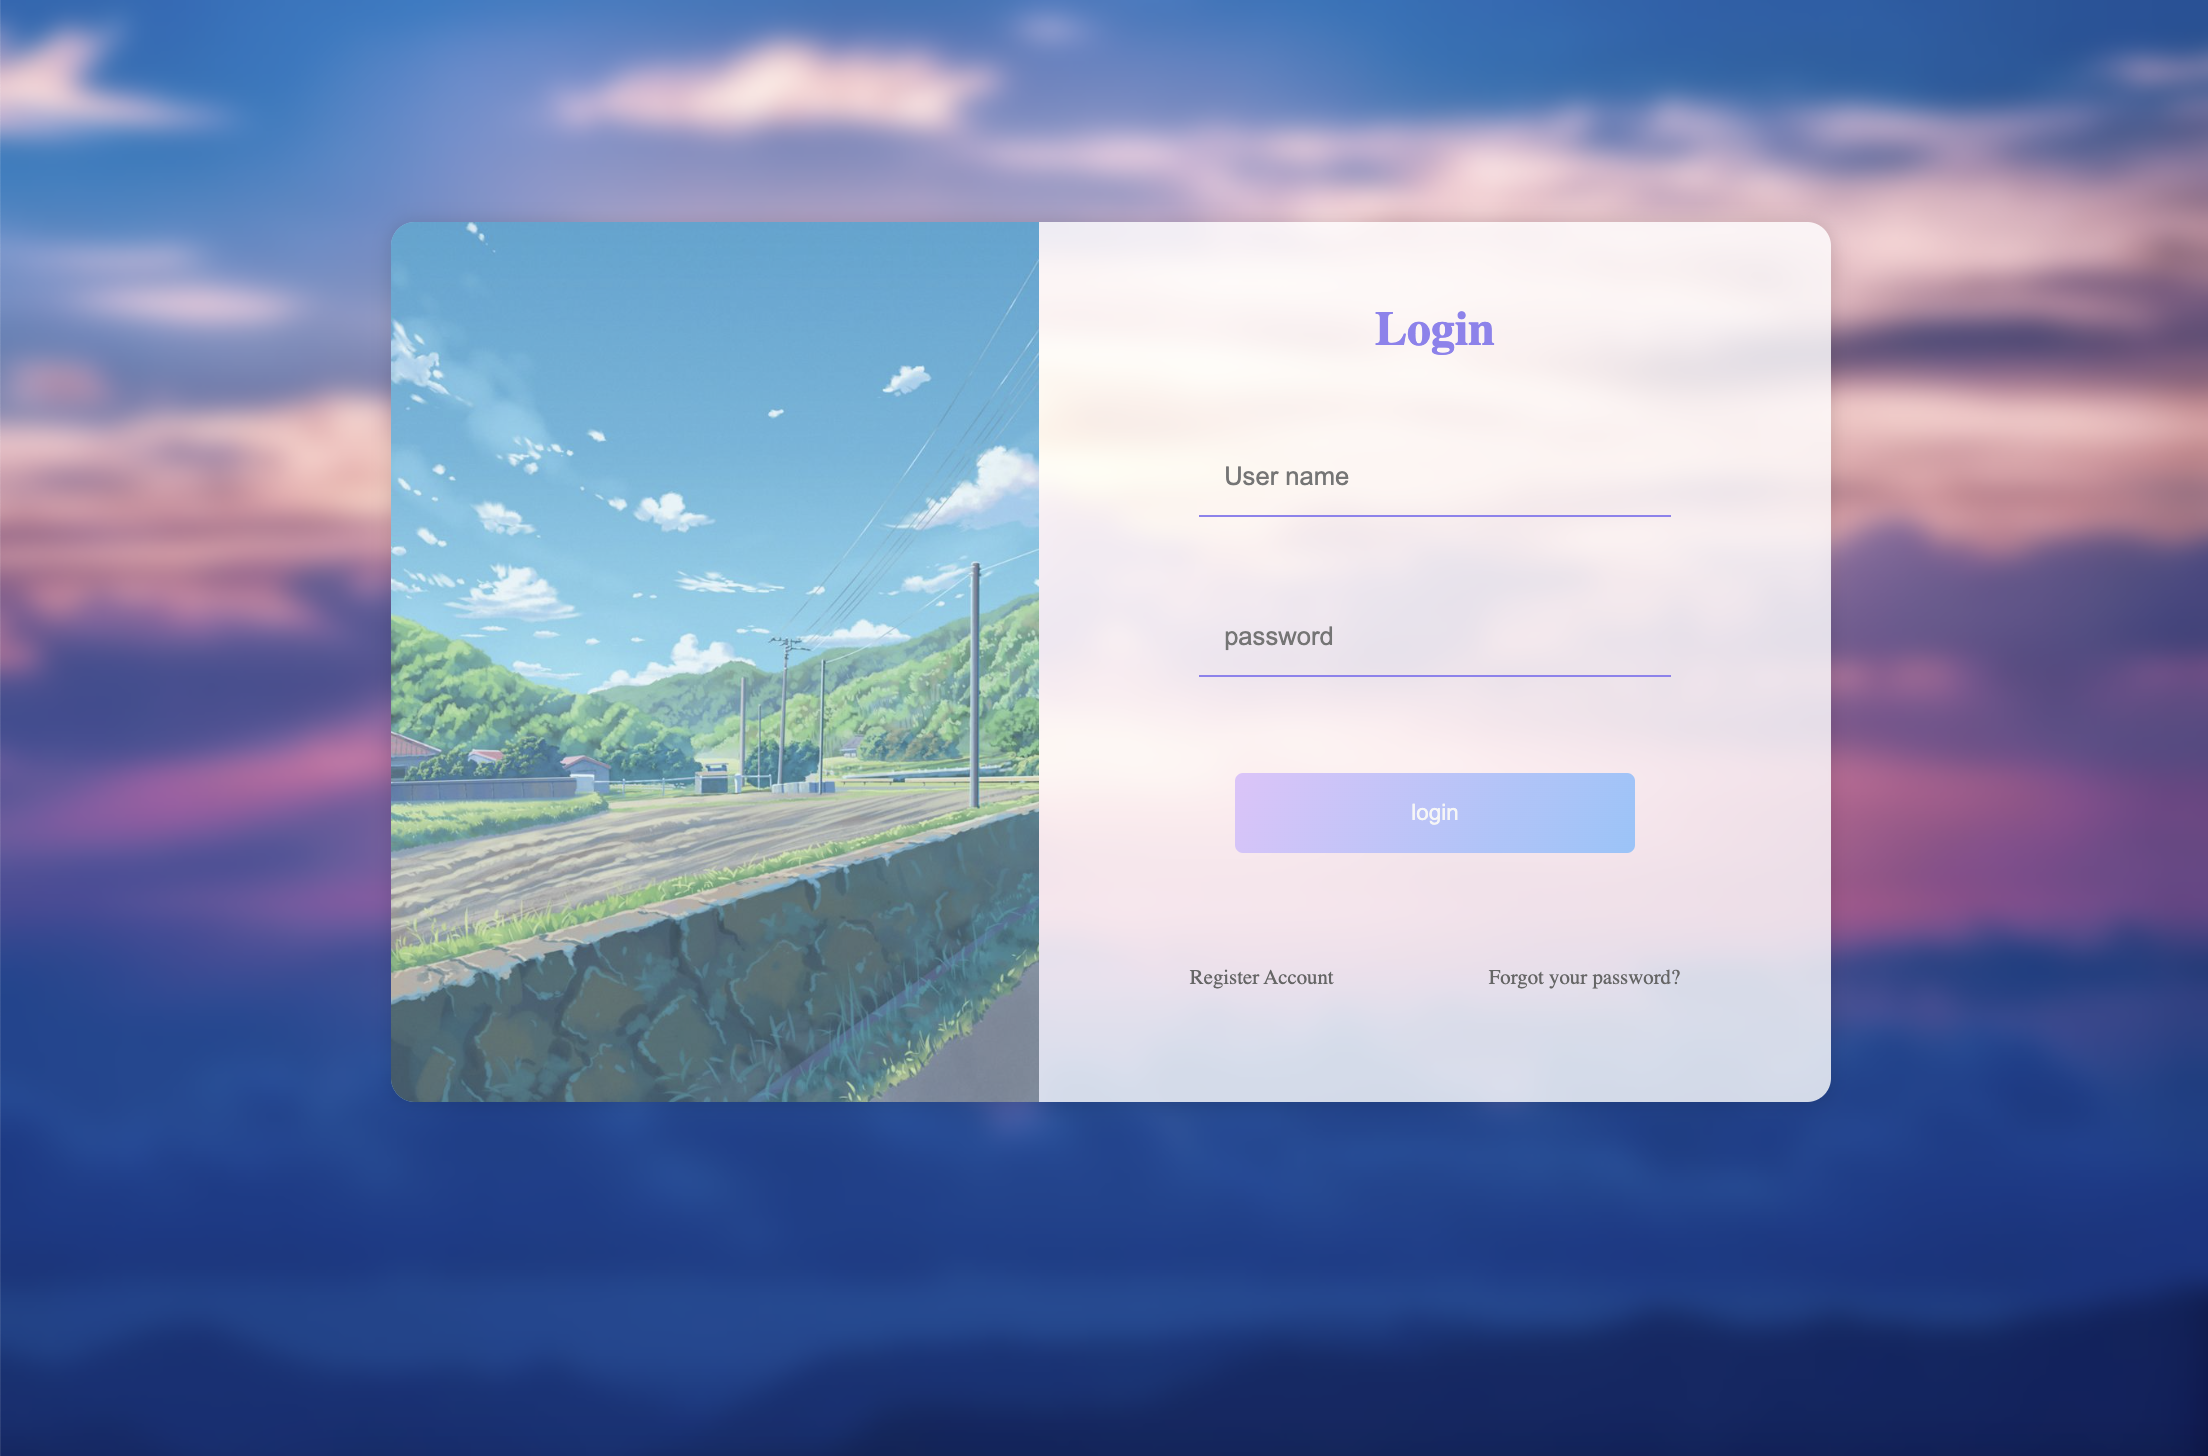
\includegraphics[width=1\linewidth]{login.png}
\caption{\label{fig:frog}login page}
\end{figure}

\begin{figure}
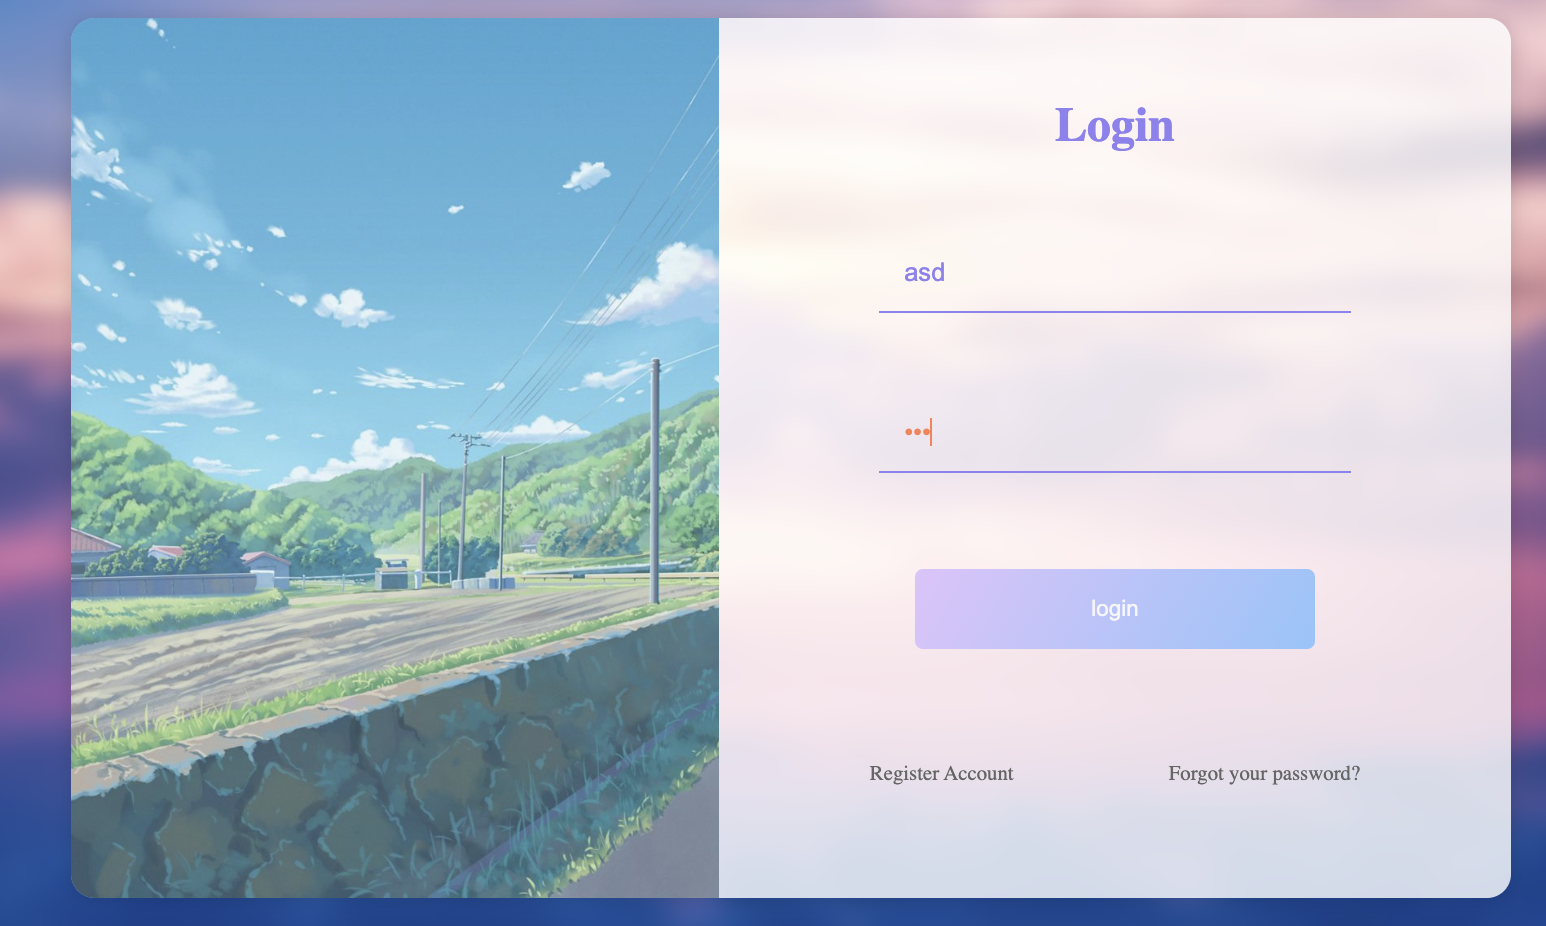
\includegraphics[width=1\linewidth]{login1.png}
\caption{\label{fig:frog}Set username and password}
\end{figure}

\begin{figure}
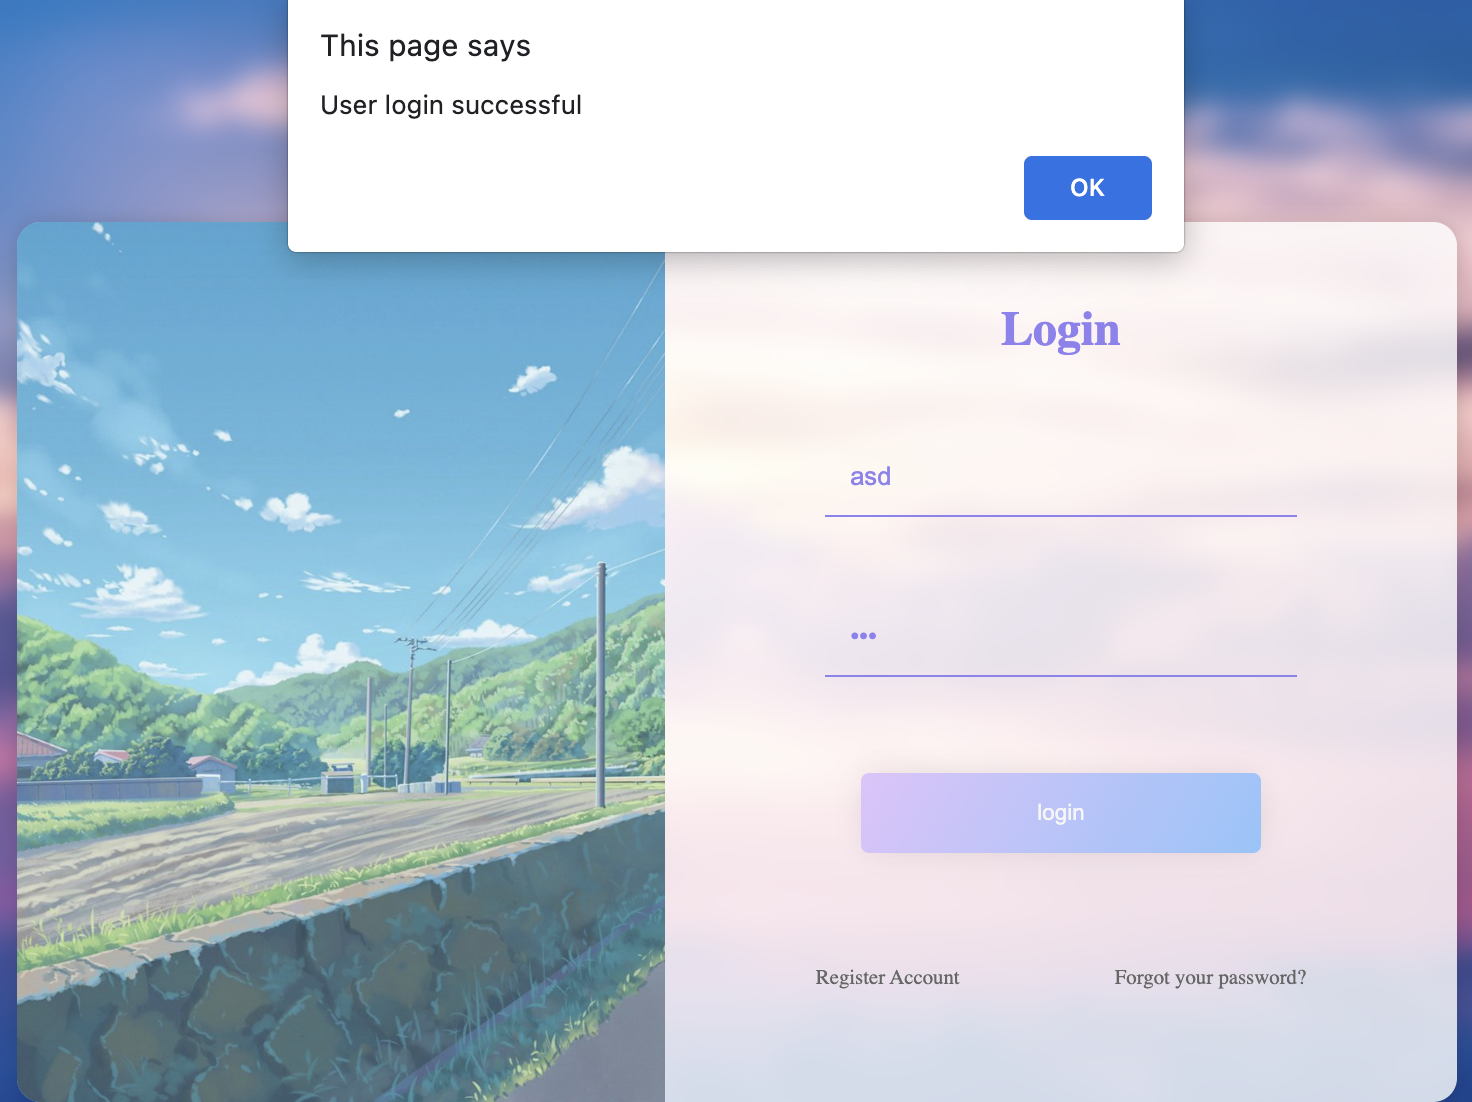
\includegraphics[width=1\linewidth]{login2.png}
\caption{\label{fig:frog}Successful}
\end{figure}

\begin{figure}
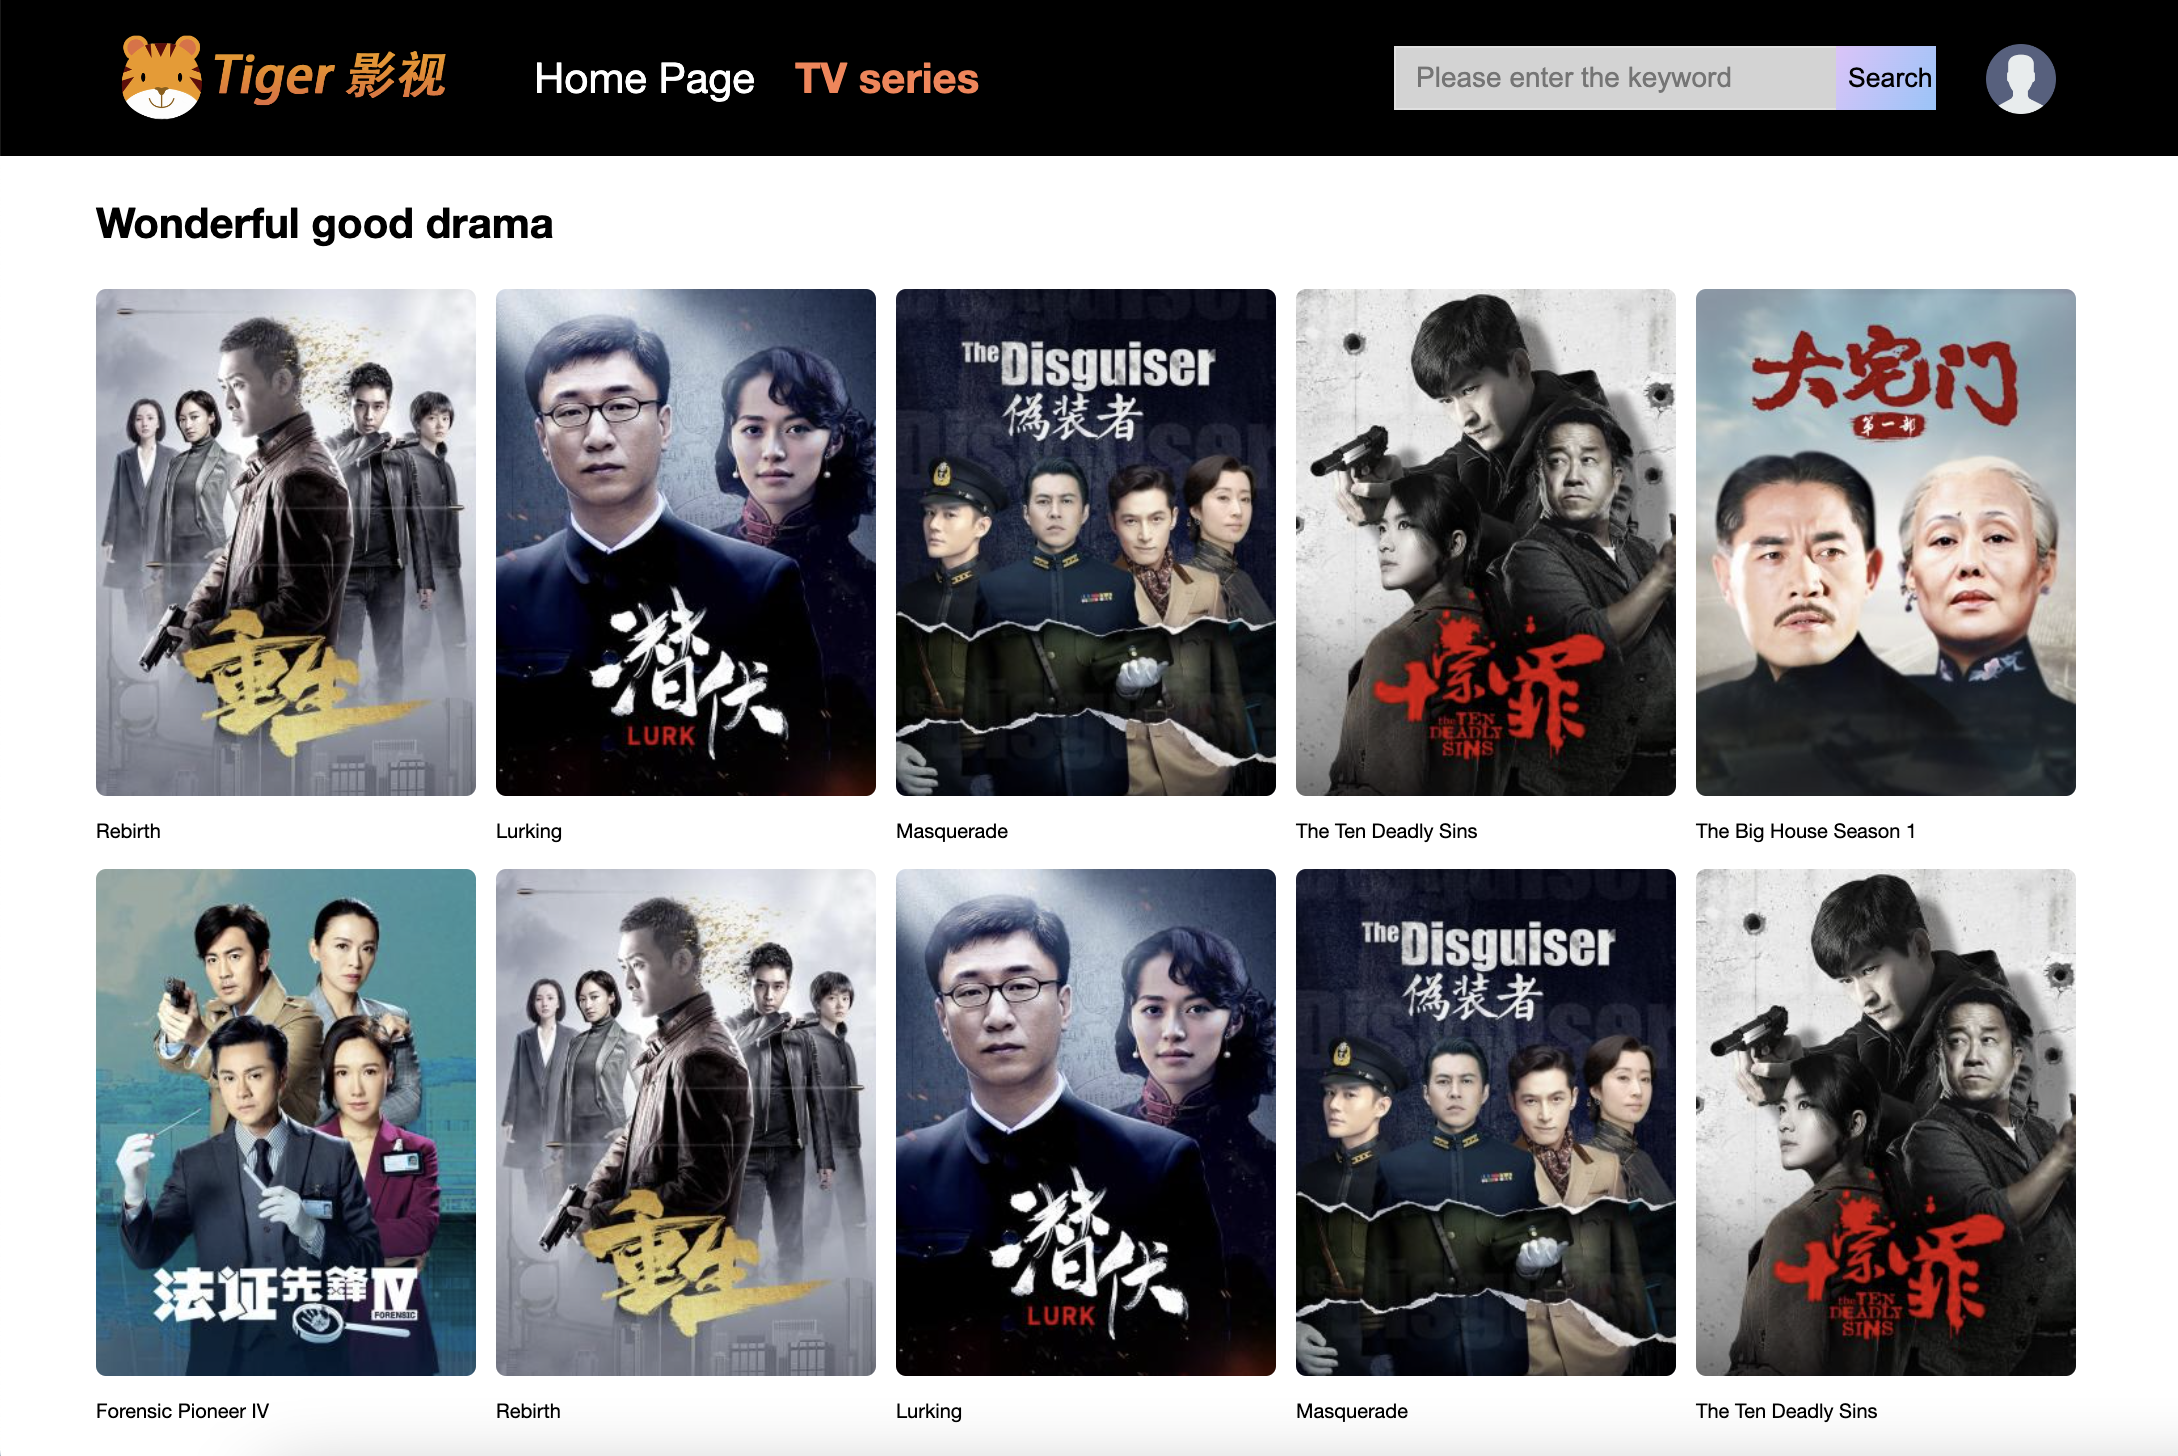
\includegraphics[width=1\linewidth]{hp.png}
\caption{\label{fig:frog}Home page}
\end{figure}

\begin{figure}
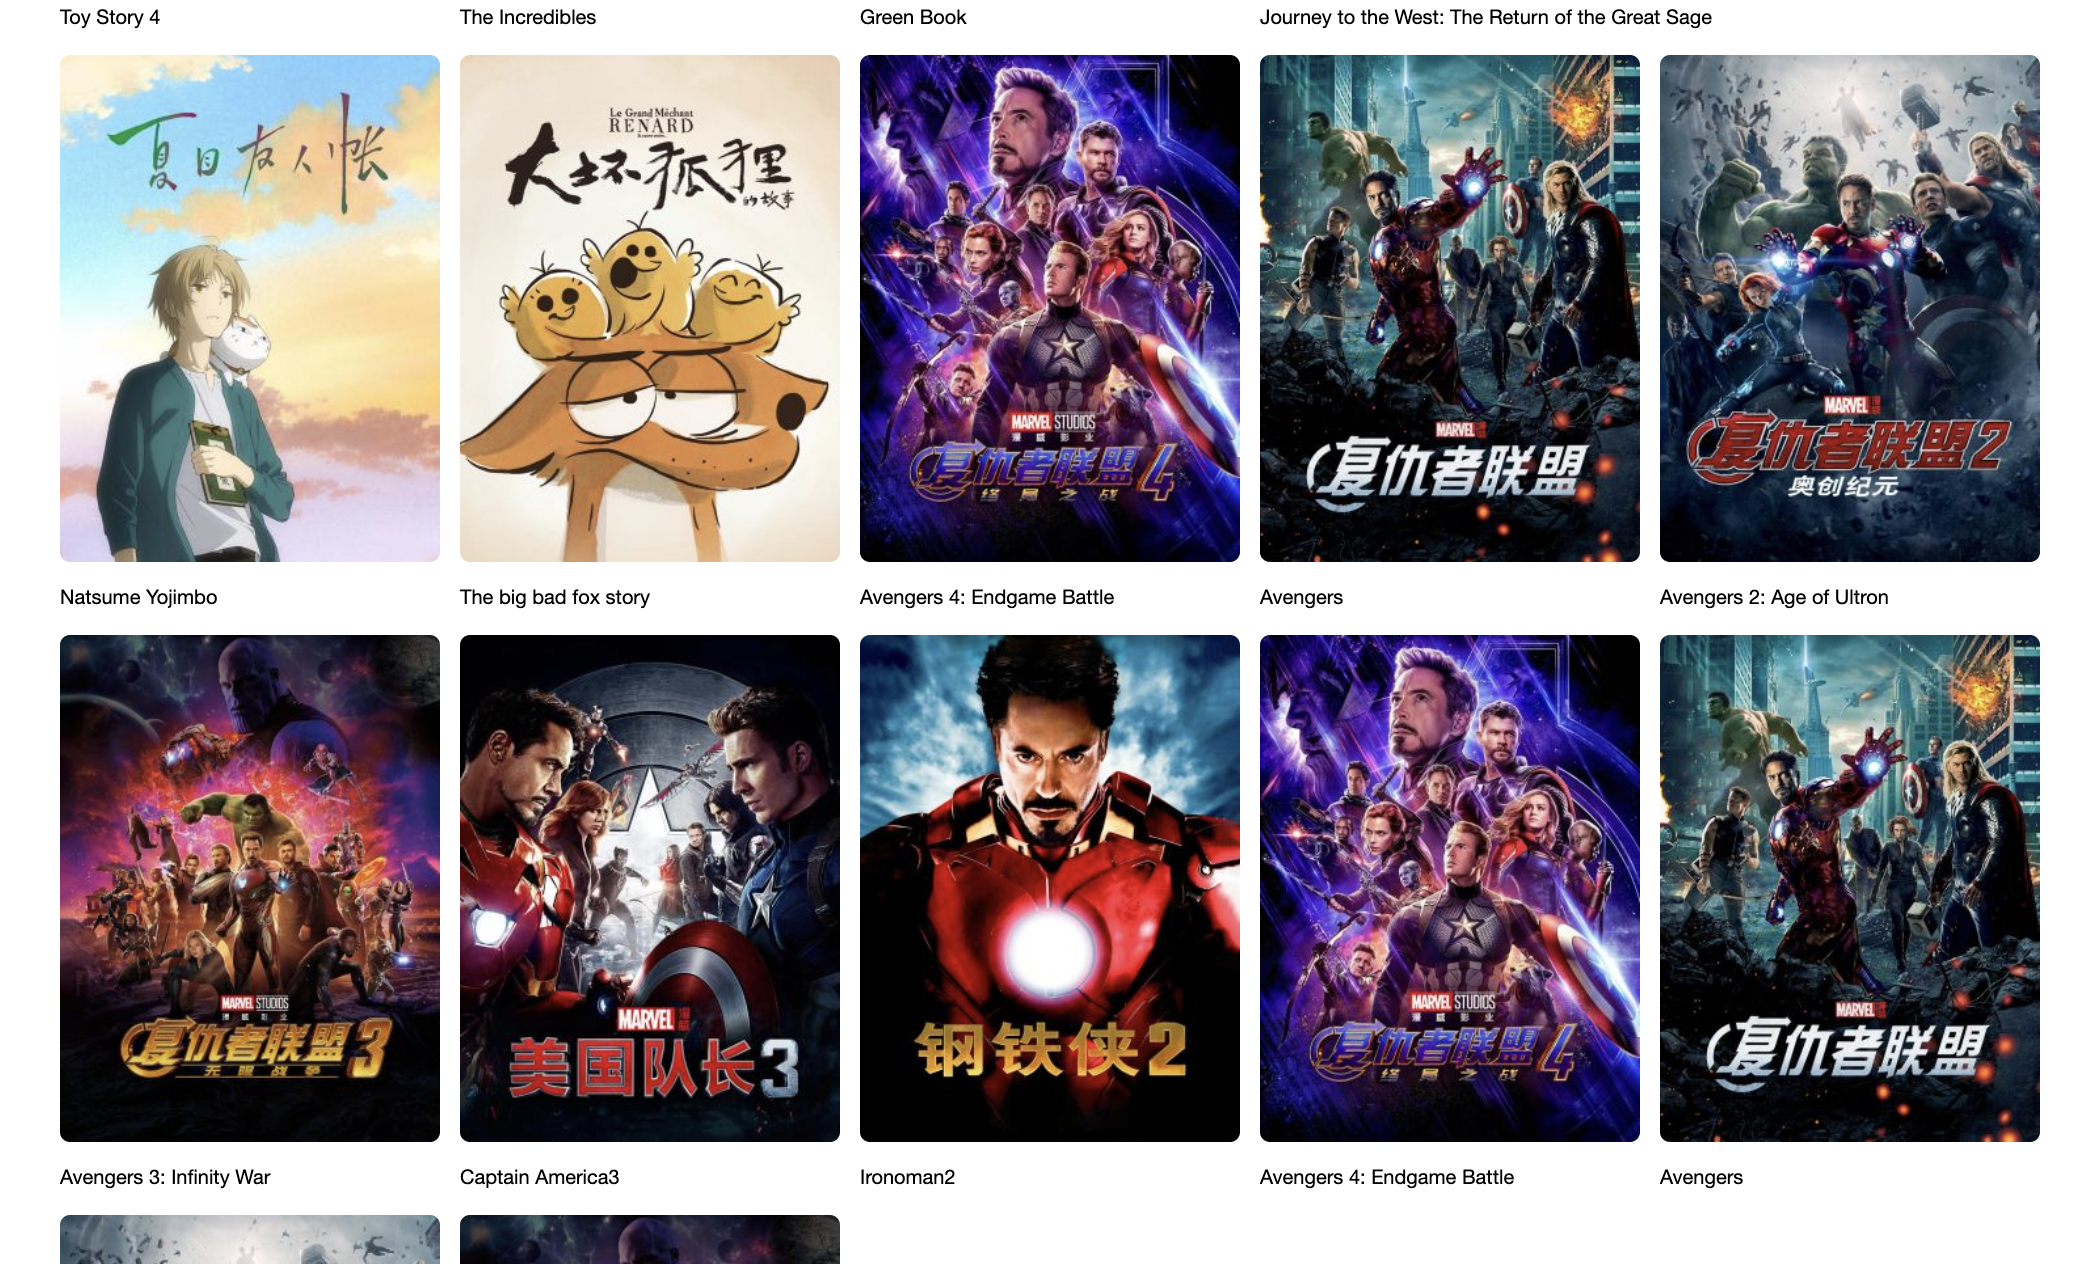
\includegraphics[width=1\linewidth]{hp1.png}
\caption{\label{fig:frog}Home page}
\end{figure}

\begin{figure}
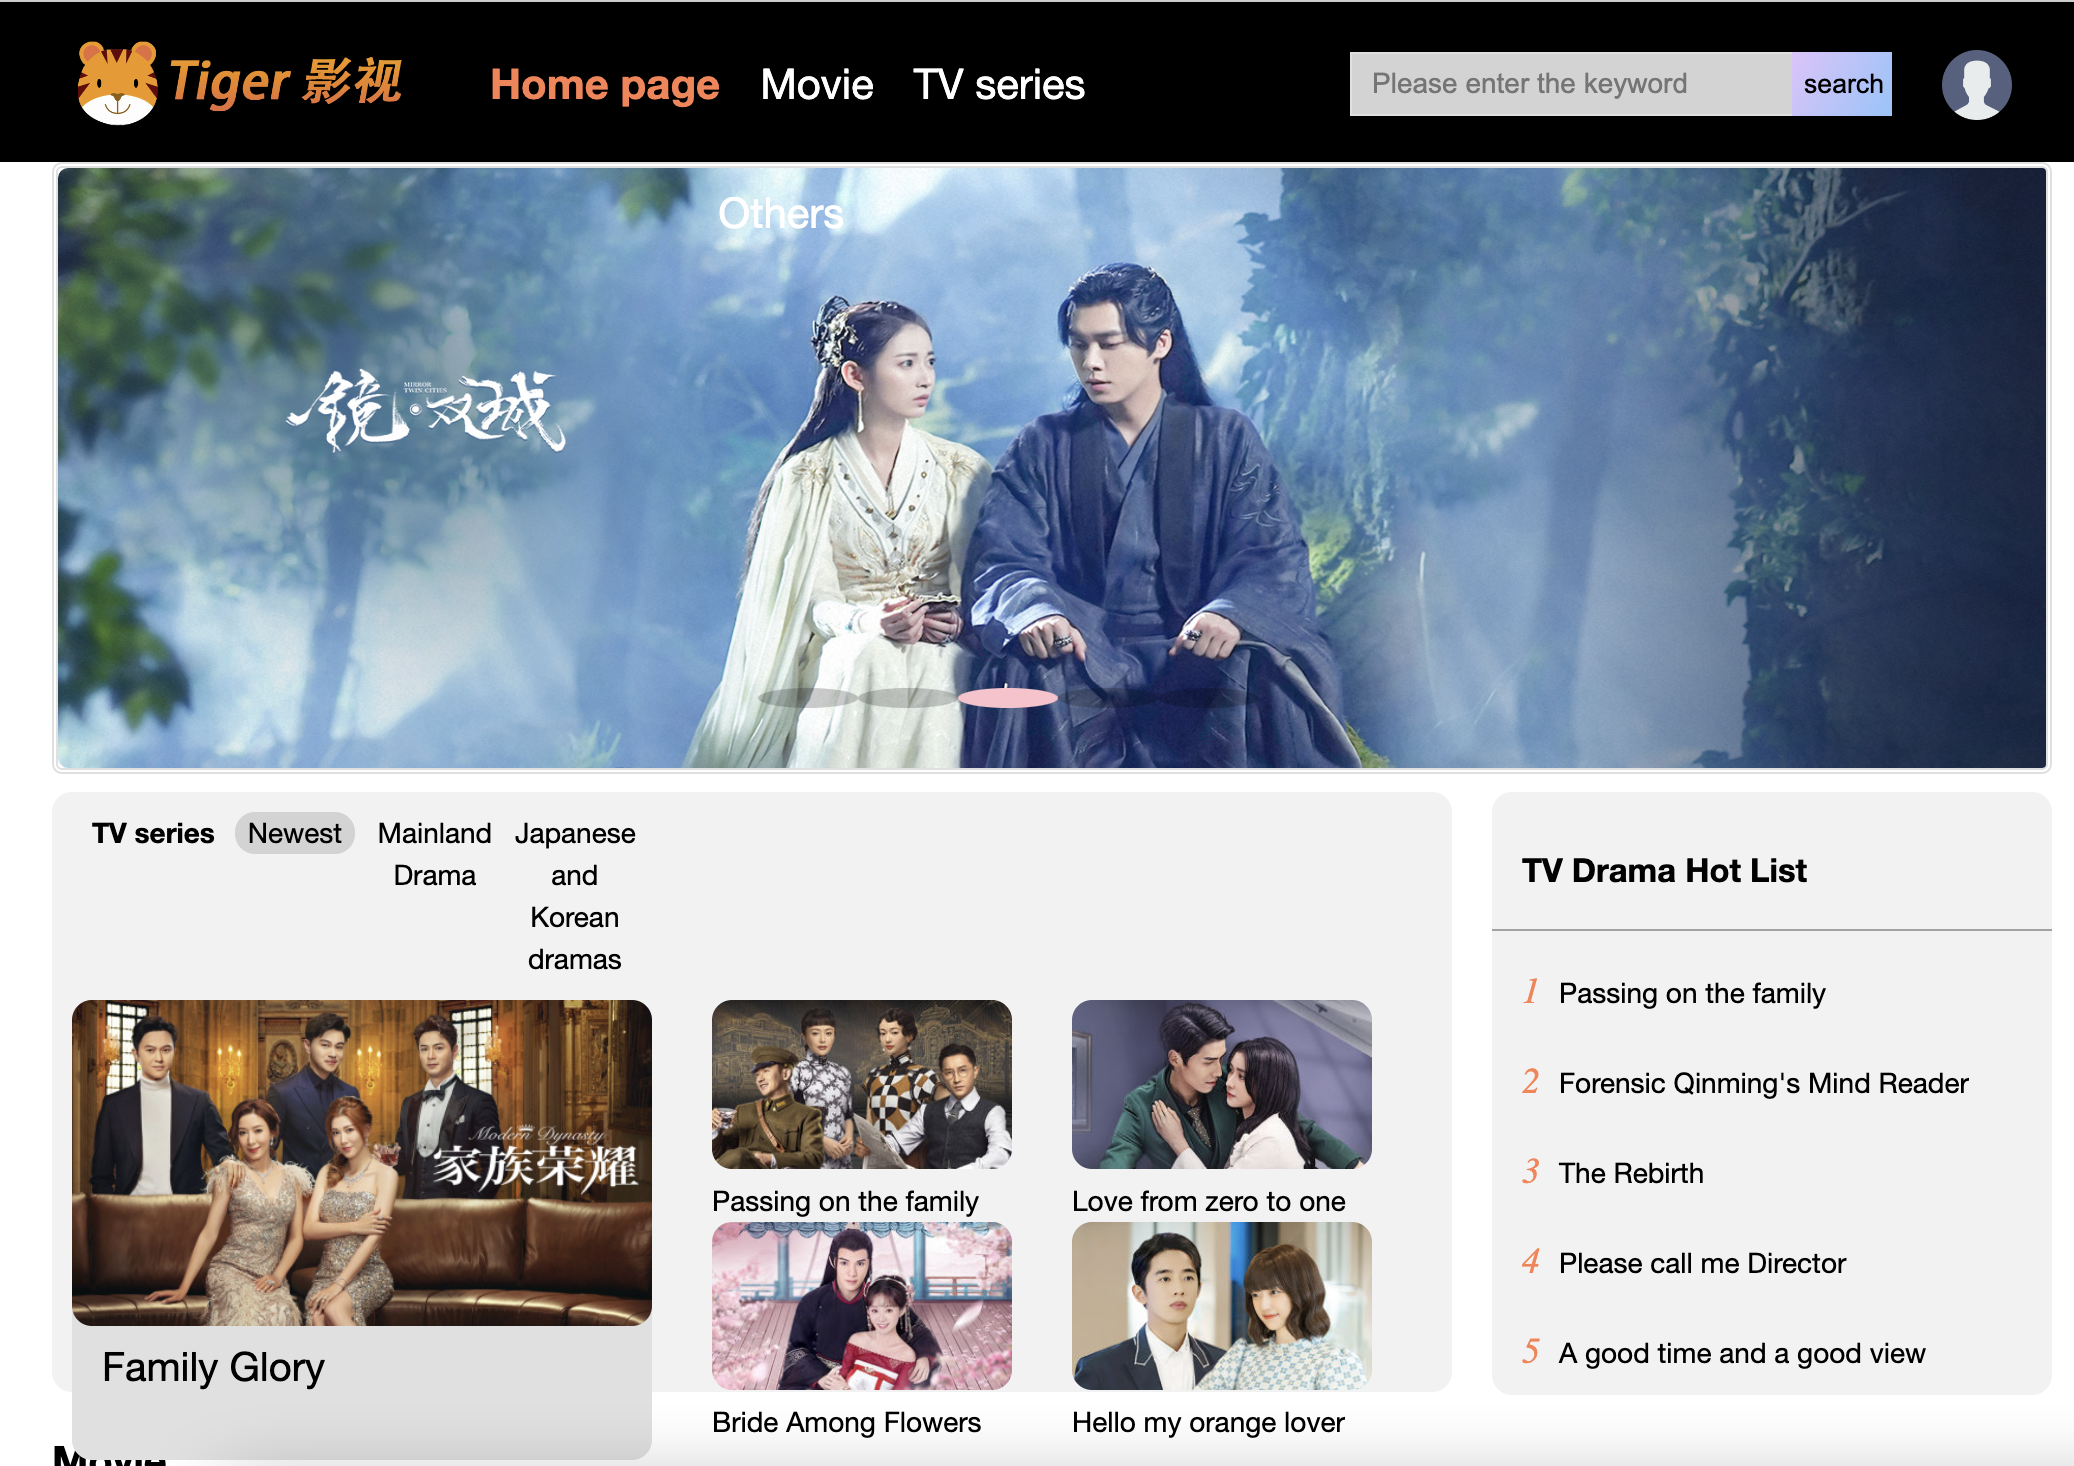
\includegraphics[width=1\linewidth]{hp2.png}
\caption{\label{fig:frog}Home page}
\end{figure}

\begin{figure}
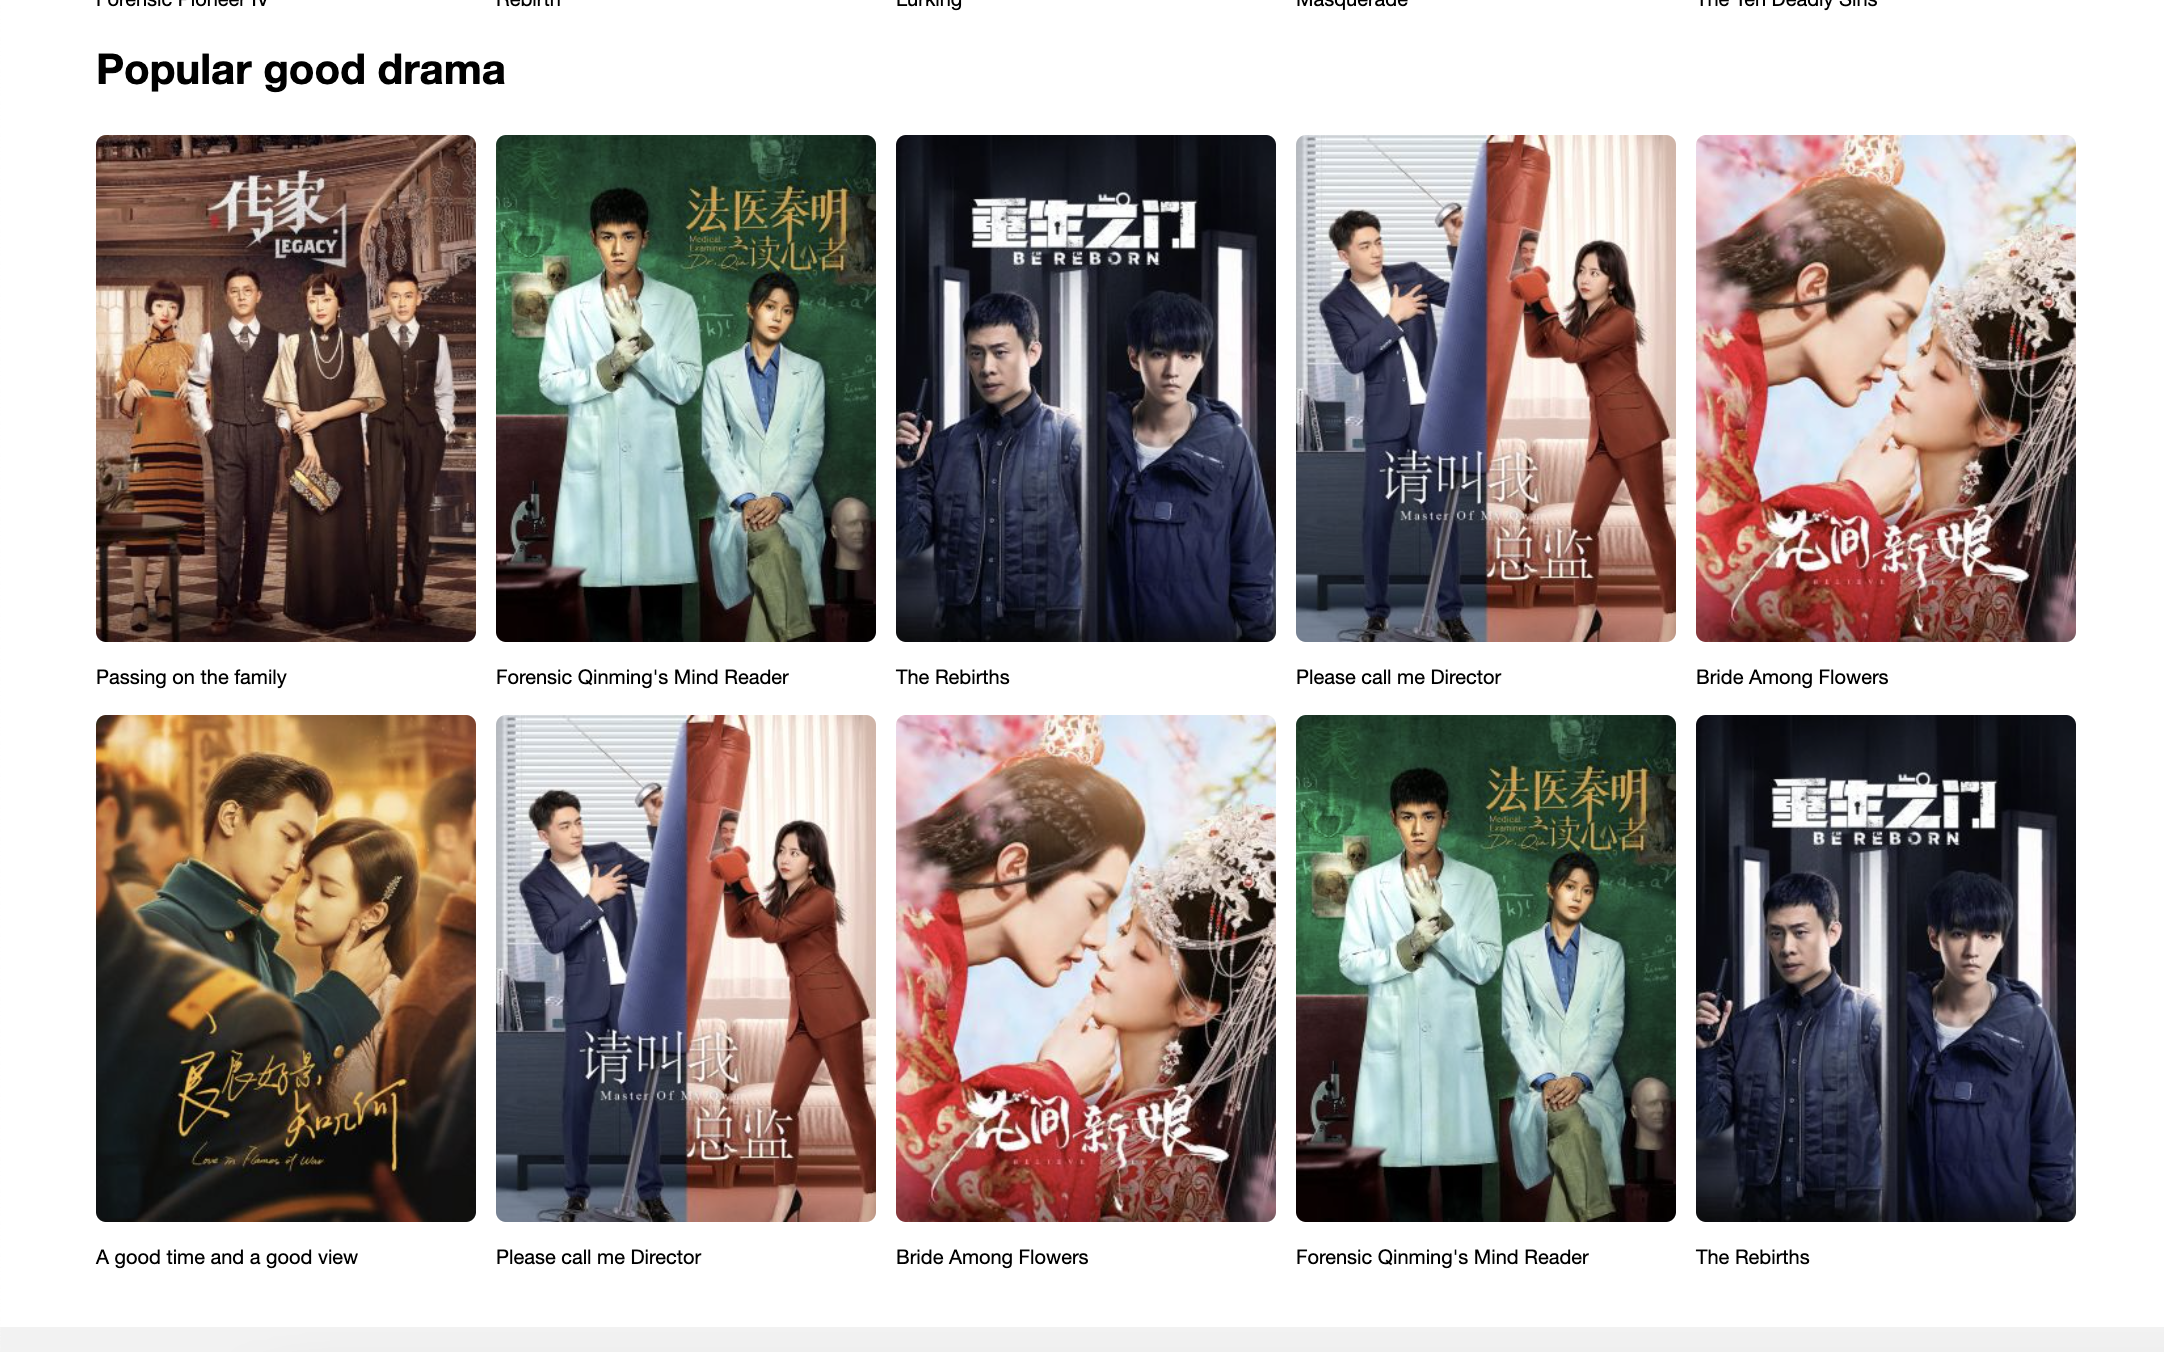
\includegraphics[width=1\linewidth]{index1.png}
\caption{\label{fig:frog}Index page}
\end{figure}

\begin{figure}
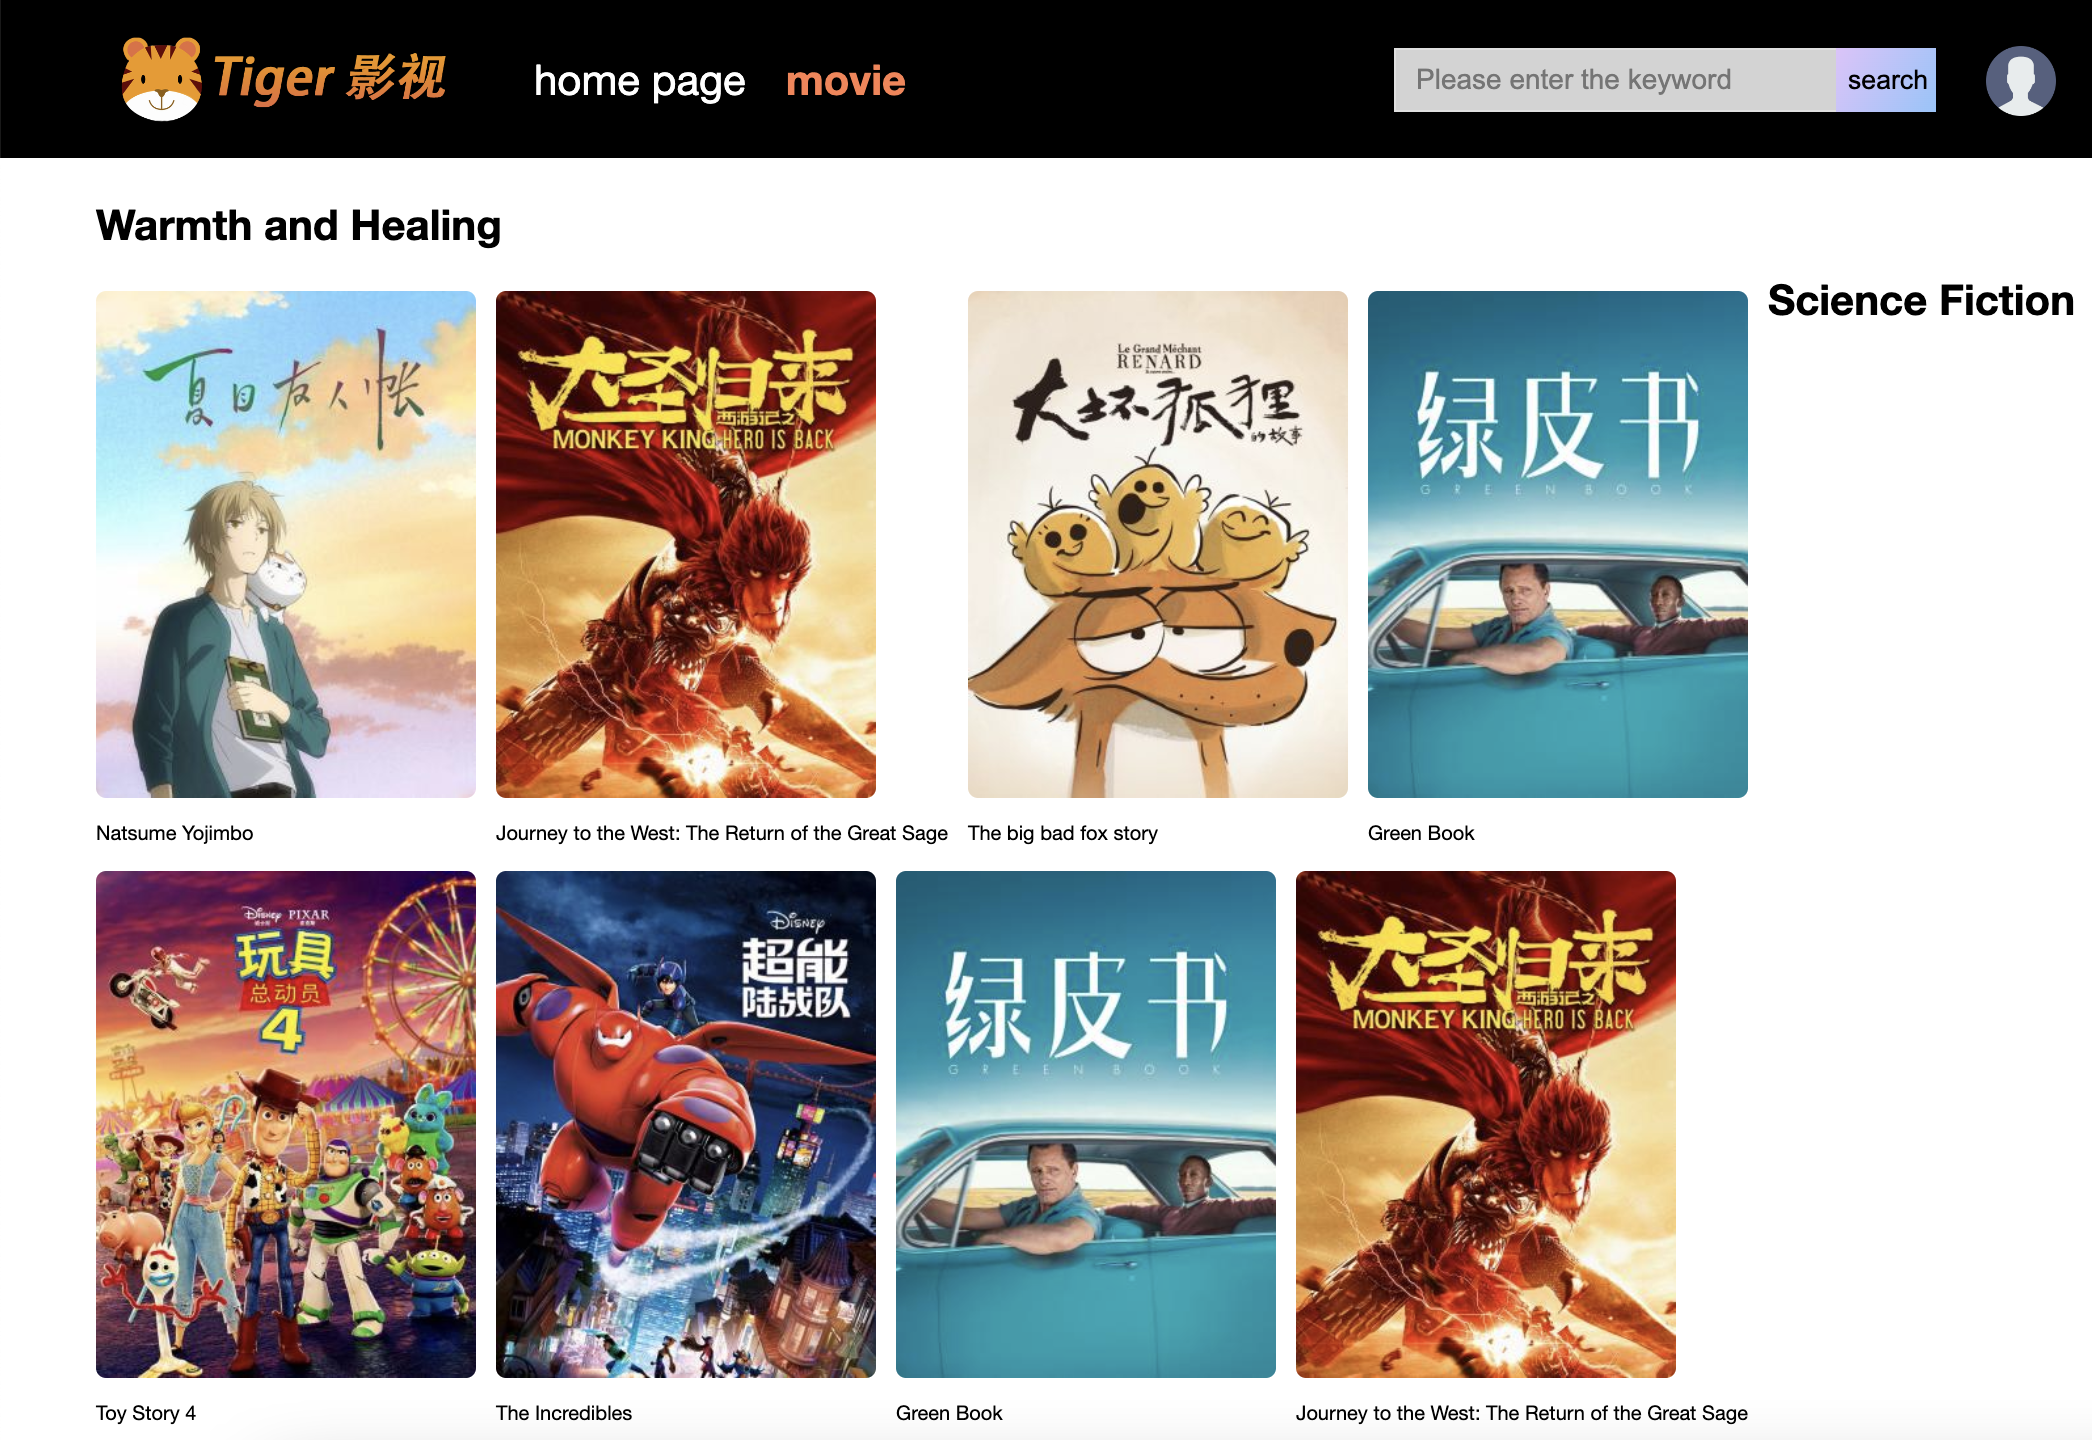
\includegraphics[width=1\linewidth]{index2.png}
\caption{\label{fig:frog}Index page}
\end{figure}

\begin{figure}
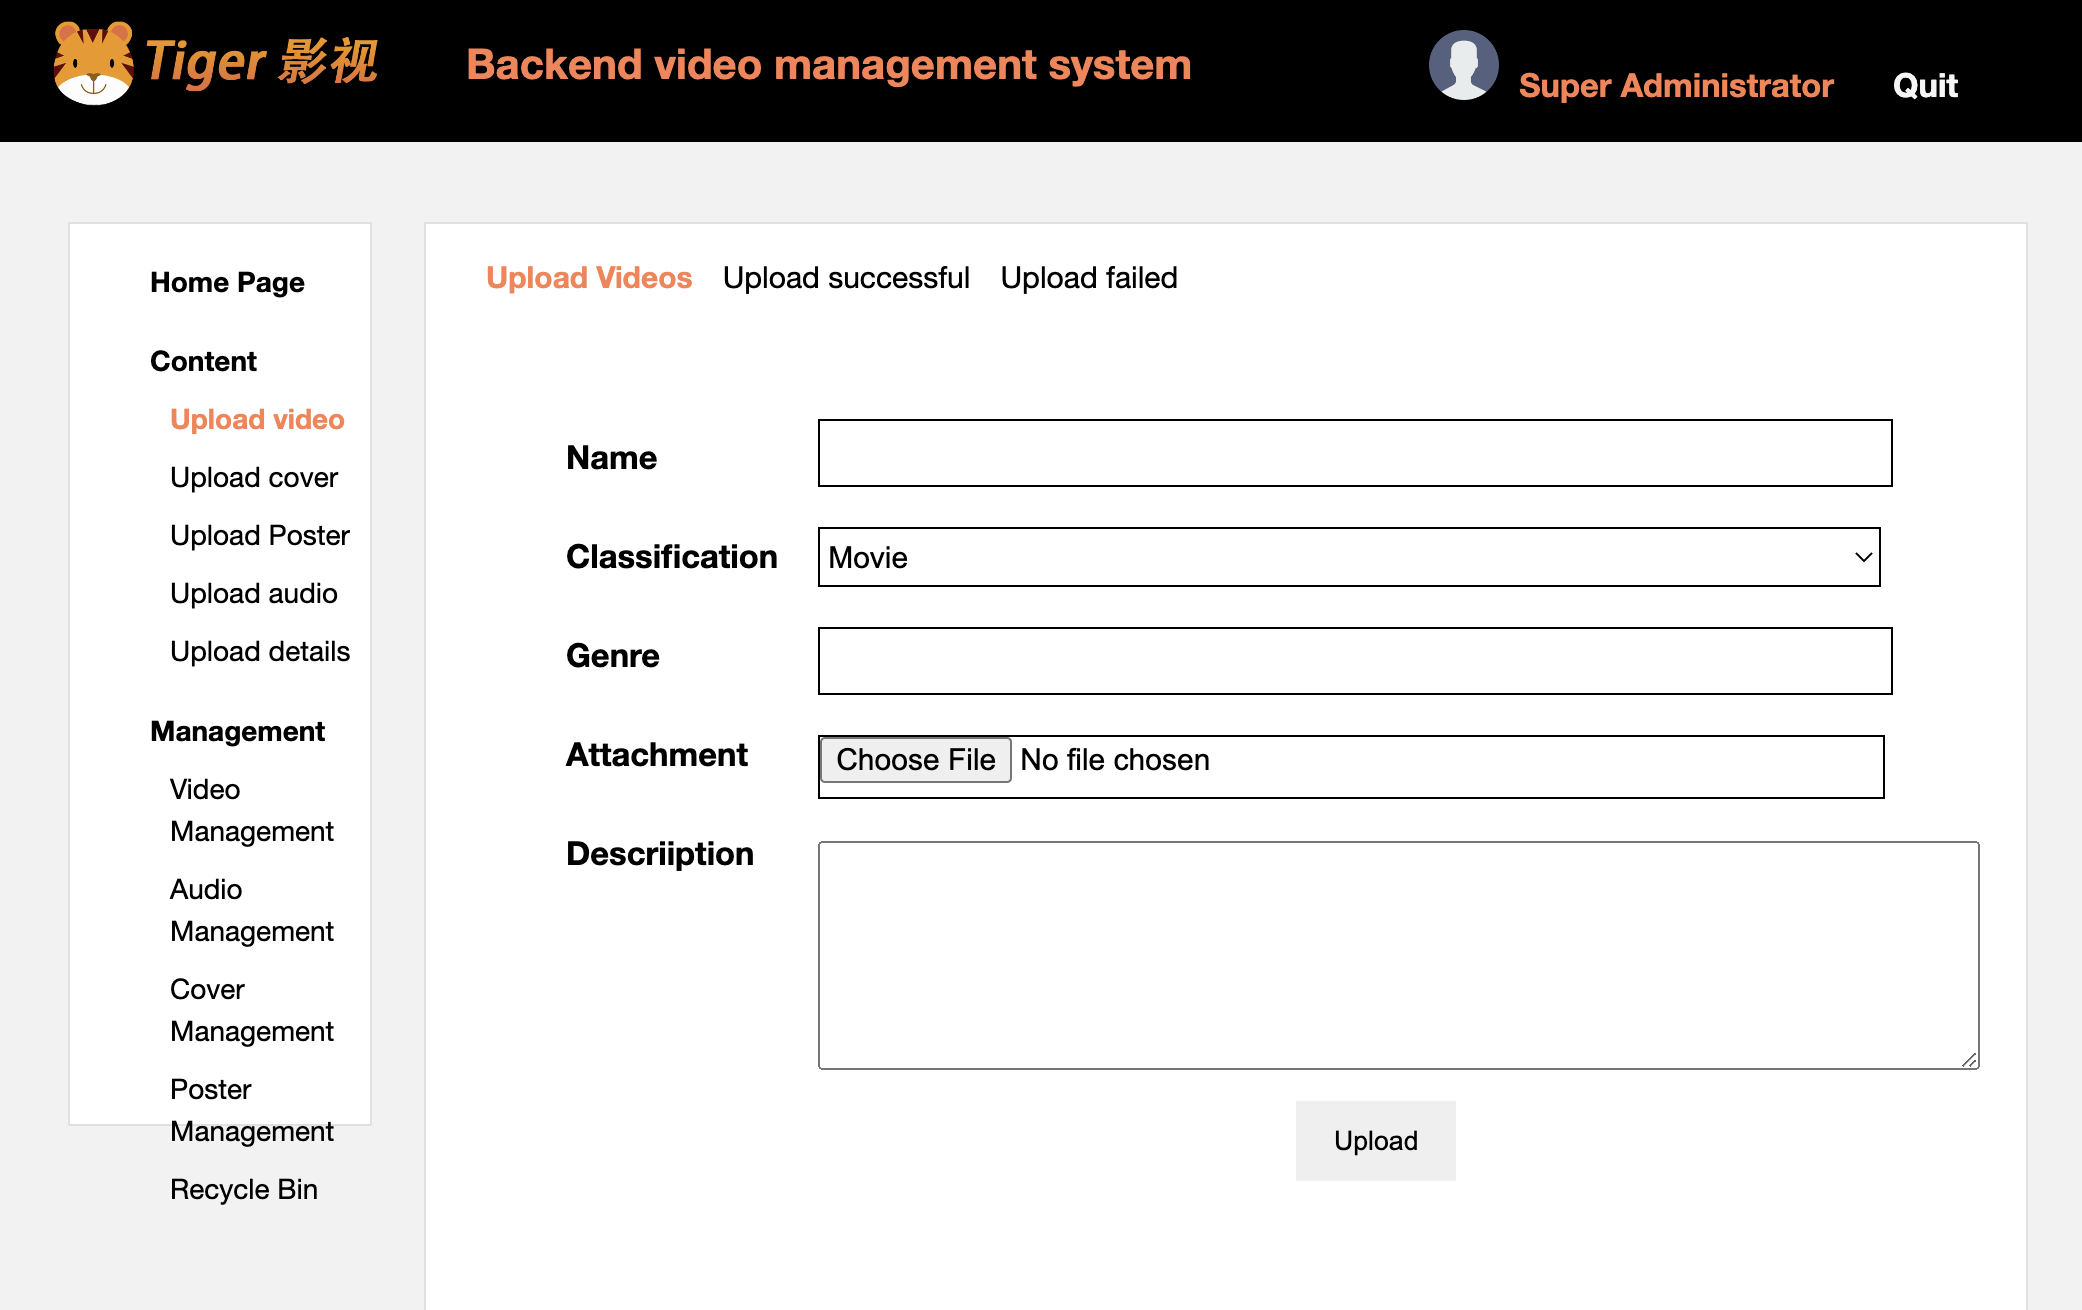
\includegraphics[width=1\linewidth]{mng.png}
\caption{\label{fig:frog}management page}
\end{figure}

\section{Screenshots}



\section{What I learned from HTML, CSS, and JavaScript}

\subsection{Advantages}
HTML, CSS, and JavaScript are three essential technologies used in web development. I have learned that they have those advantages:
HTML (Hypertext Markup Language):
\begin{itemize}
\item 	Structure: HTML provides the foundation for structuring web content. It allows you to define the hierarchy of elements, such as headings, paragraphs, lists, tables, forms, and more. This structural markup is crucial for organizing and presenting information on web pages.
\item 	Accessibility: HTML supports semantic tags, which give meaning to the content and help improve accessibility. By using appropriate semantic tags like <header>, <nav>, <main>, and <footer>, you make your website more accessible to assistive technologies and improve search engine optimization (SEO).
\end{itemize}
CSS (Cascading Style Sheets):
\begin{itemize}
\item 	Visual Styling: CSS allows you to control the visual presentation of HTML elements. With CSS, you can define colors, fonts, layouts, backgrounds, borders, and other visual properties of your web pages. It gives you the power to create visually appealing and consistent designs across your website.
\item 	Responsive Design: CSS enables responsive web design, which ensures that web pages adapt to different screen sizes and devices. Using CSS media queries and flexible layout techniques, you can create a website that is optimized for desktops, tablets, and mobile devices, providing a better user experience.
\end{itemize}
JavaScript:
\begin{itemize}
\item 	Interactivity: JavaScript is a powerful language for adding interactivity to web pages. It allows you to respond to user actions, such as clicks, form submissions, and keyboard input. With JavaScript, you can create dynamic and engaging web experiences by manipulating HTML elements, updating content in real-time, and handling user interactions.
\item 	Client-Side Processing: JavaScript runs on the client-side (in the user's web browser), which reduces the need for round trips to the server. This enables you to perform various client-side operations, such as form validation, data manipulation, calculations, and dynamic content generation. It enhances the performance and responsiveness of web applications.
\item 	Integration with APIs: JavaScript facilitates communication with server-side APIs (Application Programming Interfaces). It enables you to fetch data from external sources, such as web services or databases, using techniques like AJAX (Asynchronous JavaScript and XML) or the newer Fetch API. This integration allows you to build dynamic and data-driven web applications.
\item 	Rich Ecosystem: JavaScript has a vast ecosystem of libraries and frameworks that extend its capabilities and simplify web development. Popular frameworks like React, Angular, and Vue.js provide efficient ways to build complex and interactive web applications. Additionally, JavaScript has an active community, extensive documentation, and a wide range of resources available for learning and troubleshooting.
\end{itemize}
By combining HTML, CSS, and JavaScript, you have the power to create visually appealing, interactive, and dynamic web pages and applications. Their strengths lie in providing structure, visual styling, interactivity, and seamless integration with server-side functionality and APIs.

\subsection{Disadvantages}
While using HTML, CSS, and JavaScript I think they have some inherent weaknesses. Here are a few key weaknesses associated with each language:
HTML (Hypertext Markup Language):
\begin{itemize}
\item	Limited Interactivity: HTML is primarily a markup language and lacks advanced interactivity capabilities. While it provides the structure and semantics for web content, it requires JavaScript to handle more complex interactivity, form validation, and data manipulation.
\item	Design Limitations: HTML's design capabilities are relatively basic compared to CSS. While you can define some basic styling attributes, HTML alone is not suitable for creating complex layouts, animations, or visually rich designs. It relies on CSS for advanced styling and presentation.
\end{itemize}
CSS (Cascading Style Sheets):
\begin{itemize}
\item	Browser Compatibility: CSS may not render consistently across different web browsers. Each browser may have its own interpretation of CSS rules, leading to inconsistencies in how a website appears. Developers often need to use workarounds or browser-specific CSS code to ensure consistent rendering across browsers.
\item	Global Scope: CSS styles are applied globally by default, which can lead to unintended conflicts and style collisions when working with larger codebases. This can make it challenging to isolate and manage styles for individual components or sections of a website.
\end{itemize}
JavaScript:
\begin{itemize}
\item	Browser Dependency: JavaScript is executed by the user's web browser, and different browsers may have varying levels of support and compatibility for certain JavaScript features or APIs. Developers often need to write cross-browser compatible code or use polyfills to ensure consistent behavior across different browsers.
\item	Security Vulnerabilities: JavaScript executed in the browser has access to sensitive user information and can potentially be exploited by malicious code. Cross-site scripting (XSS) attacks and other security vulnerabilities can occur if proper security measures are not implemented.
\item	Performance Impact: Poorly optimized JavaScript code or excessive use of JavaScript can negatively impact website performance. Large JavaScript files can slow down page loading times, especially on slower connections or less powerful devices. Care must be taken to optimize and minimize JavaScript code where possible.
\item	Complexity and Learning Curve: JavaScript has a steeper learning curve compared to HTML and CSS. It is a full-fledged programming language with a wide range of concepts and features. Mastering JavaScript requires a solid understanding of programming principles, asynchronous programming, and various JavaScript frameworks and libraries.
\end{itemize}

\section{Scenario}

One scenario where the knowledge of HTML, CSS, and JavaScript can be useful is when building an e-commerce website.


In an e-commerce website, HTML provides the structure and semantic markup for the various components of the site, such as product listings, navigation menus, search bars, and checkout forms. It allows me to organize the content in a logical and accessible manner, making it easier for users to navigate and understand the website's structure.

CSS comes into play to style the e-commerce website, ensuring a visually appealing and consistent user interface. With CSS, I can define the colors, fonts, spacing, and layout of the website, creating a cohesive and professional look. CSS also enables responsive design, allowing the website to adapt and display properly on different devices, such as desktops, tablets, and mobile phones.

JavaScript adds interactivity and functionality to the e-commerce website. It allows me to implement features like product filtering and sorting, dynamic shopping carts, image sliders, and interactive forms for capturing customer information. JavaScript can also handle user interactions, such as adding items to the cart, updating quantities, and performing real-time calculations.

Furthermore, JavaScript can integrate with backend APIs to fetch and update product data, handle payment processing, and manage user authentication. This integration enables me to create a seamless and secure shopping experience for customers.
Overall, the combination of HTML, CSS, and JavaScript empowers me to build a robust and user-friendly e-commerce website. HTML provides the structure, CSS handles the visual presentation, and JavaScript adds interactivity and functionality, enabling me to create a compelling and engaging online shopping platform.

\section{References}

\url{https://blog.hubspot.com/marketing/web-design-html-css-javascript}

\url{https://www.w3schools.com/}

\url{https://www.youtube.com/results?search_query=js}



\end{document}